\section{Parallelized Solvers}
\frame{\tableofcontents[currentsection, currentsubsection]}

\subsection{Introduction}

\frame{ \frametitle{Introduction}
\begin{itemize}
\item Algorithmic improvement to $\ell_1$ minimization provided significant speed boost, but still not enough.
\item This section presents parallelized implementations of the face pipeline
\item There is ample parallelism available in the pipeline
\item Leverage the high levels of concurrency available in multi-core CPU and GPU architectures.
\end{itemize}
}

\subsection{Hardware Overview}
\frame{ \frametitle{CPU Hardware Overview}
\begin{itemize}
\item Large ammounts of cache (on-chip memory) compared to GPU
\item High clock speeds compared to GPU
\end{itemize}
}

\frame{ \frametitle{CPU Hardware Overview}
\begin{itemize}
\item Intel E5530, Dual-socket, quad-core Xeon
\item Each core has a private 32\,KiB L1 data cache 
\item Each core has a private 256\,KiB L2 cache.
\item Each chip has a shared 8\,MiB L3 cache.
\end{itemize}
}

\frame{ \frametitle{CPU Hardware Overview}
\begin{itemize}
\item Each of the 8 cores has a vector processor unit (SSE) that
can perform 4 single precision floating point operations concurrently.
\item Two levels of concurrency: {\em core-level} and {\em SSE-level}
\end{itemize}
}

\frame{ \frametitle{GPU Hardware Overview}
\begin{itemize}
\item High memory bandwidth compared to CPU
\item Much higher degree of concurrency compared to CPU
\end{itemize}
}
 
\frame{ \frametitle{GPU Hardware Overview}
\begin{itemize}
\item Single GTX480 GPU chip on PCIe expansion card
%\item Nvidia GTX480 programmed in C for CUDA
\item Up to 16 {\em streaming multiprocessors} (SMs).
\item Each SM can execute 64 (two warps of 32 threads) floating point
operations concurrently.
\item Two levels of concurrency: {\em SM-level} and {\em thread-level} 
\end{itemize}
}


\frame{ \frametitle{GPU Hardware Overview}
\begin{itemize}
\item Each SM has 64 KiB of private L1 cache
\item The chip has 768 KiB of shared L2 cache
\end{itemize}
}

\newcommand{\tempscale}[0]{0.7}
\frame{ \frametitle{CPU and GPU cache comparison}
\centering
The larger algorithm data structures: \\
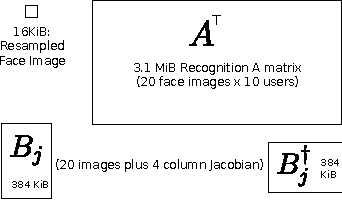
\includegraphics[scale=\tempscale]{../figures_ijcb/arrays.pdf} \\
The caches on a E5530 CPU: \\
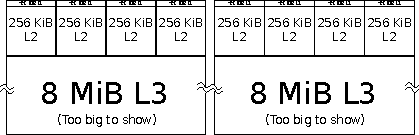
\includegraphics[scale=\tempscale]{../figures_ijcb/cpu_caches.pdf} \\
The caches on a GTX480 GPU: \\
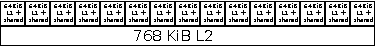
\includegraphics[scale=\tempscale]{../figures_ijcb/gpu_caches.pdf} \\
}

%\frame{ \frametitle{Limitations of CUDA programming model}
%}

\frame{ \frametitle{Parallelism in the recognition stage}
For Recognition stage:
\begin{itemize}
\item Single large $\ell_1$ minimization problem
\item Only one level of parallelism available: {\em pixel-level}
\end{itemize}
}

\frame{ \frametitle{Parallel implementation of the recognition stage}
\begin{itemize}
\item Most operations map directly onto calls in the BLAS API.
\item On the CPU, Intel's MKL BLAS can exploit both levels of concurrency on the CPU.
\item On the GPU, Nvidia's CUBLAS exploits both levels of concurrency on the CPU.
\item On the CPU, the remaining operations can be parallelized via manual threading (via OpenMP),
and automatic vectorization (via the Intel ICC compiler).
\item On the GPU, the remaining operations can be parallelized manually as CUDA kernels.
\end{itemize}
}

\frame{ \frametitle{Parallelism in the alignment stage}
For Alignment stage:
\begin{itemize}
\item Many relatively small $\ell_1$ minimization problems that are solved repeatedly
\item Two levels of parallelism available: \emph{problem-level} and \emph{pixel-level}
\item $\ell_1$ minimization is interleaved with image rewarping.
\end{itemize}
}

\frame{ \frametitle{Parallel implementation of the alignment stage}
\begin{itemize}
\item TODO
%\item Most operations map directly onto calls in the BLAS API.
%\item On the CPU, Intel's MKL BLAS can exploit both levels of concurrency on the CPU.
%\item On the GPU, Nvidia's CUBLAS exploits both levels of concurrency on the CPU.
%\item On the CPU, the remaining operations can be parallelized via manual threading (via OpenMP),
%and automatic vectorization (via the Intel ICC compiler).
%\item On the GPU, the remaining operations can be parallelized manually as CUDA kernels.
\end{itemize}
}

\subsection{Parallelization of Recognition Stage}
\frame{ \frametitle{Implementation via BLAS, OpenMP, CUBLAS} Fairly straightforward.}
\frame{ \frametitle{Benchmarks on public datasets} Speed improvements!  In fact, no longer the most expensive
part of the pipeline}
\frame{ \frametitle{Scalability} Discuss effect of CPU cache, better scalability of GPU for huge problems}
\subsection{GPU Alignment Parallelization}
\frame{ \frametitle{Microbenchmarks} Motivate single solver per core for alignment}
\frame{ \frametitle{GPU Implementation} Discuss implementation challenges}
\frame{ \frametitle{GPU Implementation} Performance optimization, array storage}
\frame{ \frametitle{GPU Implementation} Performance optimization, tuning}
\frame{ \frametitle{GPU Implementation} Performance optimization, numerical precision}
\frame{ \frametitle{GPU Implementation} Discuss implementation challenges}
\frame{ \frametitle{Benchmarks} Code runs fast on public datasets.}
\subsection{CPU Alignment Parallelization}
\frame{ \frametitle{Microbenchmarks} Motivate single solver per core}
\frame{ \frametitle{GPU Implementation} Discuss implementation challenges}
%\subsection{Recap}
\frame{ \frametitle{Existing Architectures are already fast} CPU and GPU architectures competitive, and
both benefit dramatically from proper parallelization.  Implementation on GPU much more painful; no SM level
libraries}
\frame{ \frametitle{Improving hardware architectures} CPU/GPU hybrids: Intel Knight's Corner and AMD's APU}

